\section{EODP-TS-L1C. Level-1C processing}
\label{sec:l1c}

\subsection{Objective}
The test validates the L1C module.
The L1C projects the L1B radiances onto the MGRS grid \cite{atbd}. The steps are the following.
\begin{enumerate}
\item Build a 2D spline interpolant of the L1B radiance as a function of latitude and longitude (\texttt{bisplrep}).
\item Convert every L1B coordinate into an MGRS tile with a precision of 100~m and keep the unique tiles.
\item Convert each tile back to latitude and longitude. The \texttt{mgrs} library \cite{mgrs} returns the south-west corner of the tile.
\item Evaluate the interpolant at these coordinates (\texttt{bisplev}). The result is the L1C radiance.
\end{enumerate}

\subsection{Inputs and configuration}
The inputs are the geolocation of the GM in \texttt{input/gm\_alt100\_act\_150} and the L1B radiances in \texttt{input/l1b\_output}.
Both are matrices of 100 lines by 150 columns.
The MGRS precision is 3, which gives tiles of 100~m.

\subsection{Execution}
The script \texttt{harness/EODP-TS-L1C/test\_l1c.py} runs the L1C with both input folders separated by a comma.
The L1C output is a list of points. Its order changes in each run because the tiles are stored in a Python set.
For this reason each reference point is matched with the closest output point before the comparison.

\subsection{Results}

\subsubsection{Cross-validation}
Table~\ref{tab:l1c_crossval} shows the comparison.
The number of points is the same. Every reference point has an output point at zero distance, and the radiances are identical.

\begin{table}[H]
\centering
\small
\caption{L1C cross-validation after matching the points by coordinates.}
\label{tab:l1c_crossval}
\begin{tabular}{lccccc}
\toprule
Band & Points ref. & Points output & Max. distance [m] & Max. rel. diff. [\%] & Result \\
\midrule
VNIR-0 & 3129 & 3129 & $0$ & $0$ & Pass \\
VNIR-1 & 3129 & 3129 & $0$ & $0$ & Pass \\
VNIR-2 & 3129 & 3129 & $0$ & $0$ & Pass \\
VNIR-3 & 3129 & 3129 & $0$ & $0$ & Pass \\
\bottomrule
\end{tabular}

\end{table}

\subsubsection{L1B and L1C grids}
Figure~\ref{fig:l1c_grids} shows both grids in the same plot.
The L1B grid follows the geometry of the sensor. It is tilted with respect to the meridians because of the orbit inclination.
The L1C grid is regular in UTM coordinates. Its points are aligned with the north and the east.
The L1C grid is coarser. There are 3129 L1C points against 15000 L1B points.

\begin{figure}[H]
\centering
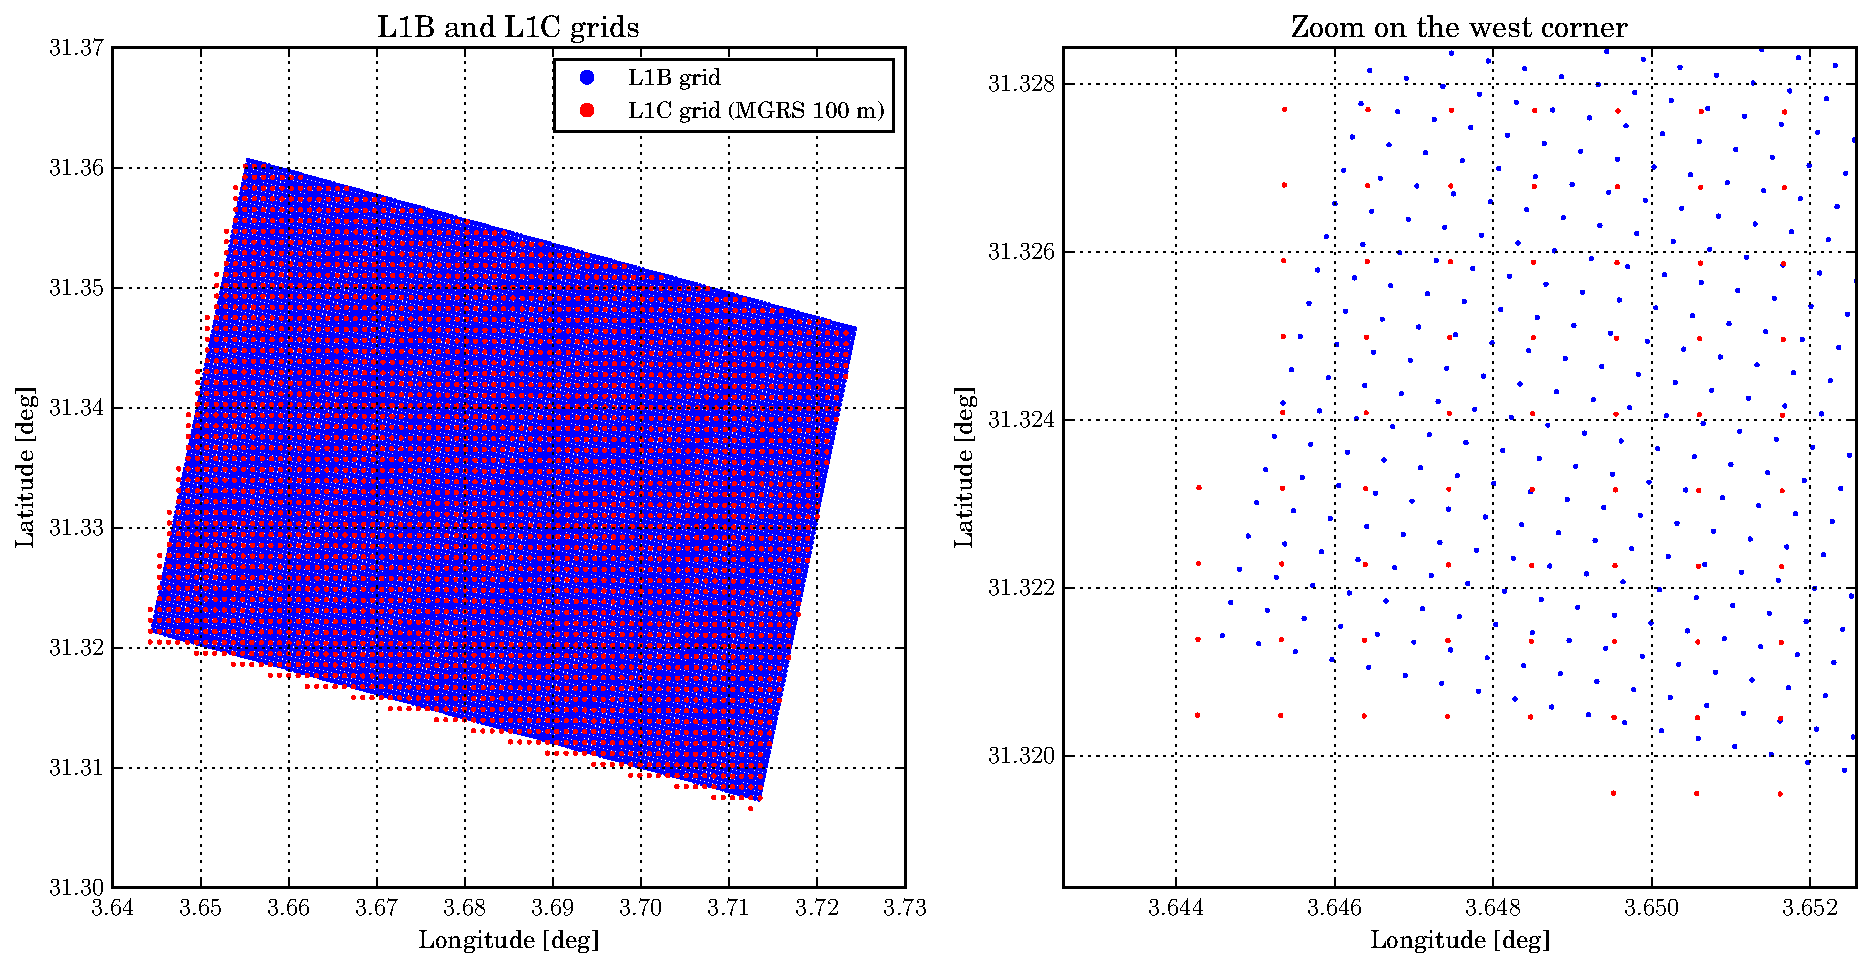
\includegraphics[width=\textwidth]{l1c_grids}
\caption{L1C. L1B and L1C grids. Full scene on the left and zoom on the west corner on the right.}
\label{fig:l1c_grids}
\end{figure}

\subsubsection{Ground sampling distance}
The GSD of the L1B is the distance on ground between consecutive pixels.
It is computed with the Haversine formula along the central line (ACT) and the central column (ALT).
Table~\ref{tab:l1c_gsd} and Figure~\ref{fig:l1c_gsd} show the result.

\begin{table}[H]
\centering
\caption{L1B ground sampling distance.}
\label{tab:l1c_gsd}
\begin{tabular}{lccc}
\toprule
Direction & Mean [m] & Min. [m] & Max. [m] \\
\midrule
ACT & 45.16 & 45.16 & 45.16 \\
ALT & 45.29 & 45.28 & 45.29 \\
\bottomrule
\end{tabular}

\end{table}

\begin{figure}[H]
\centering
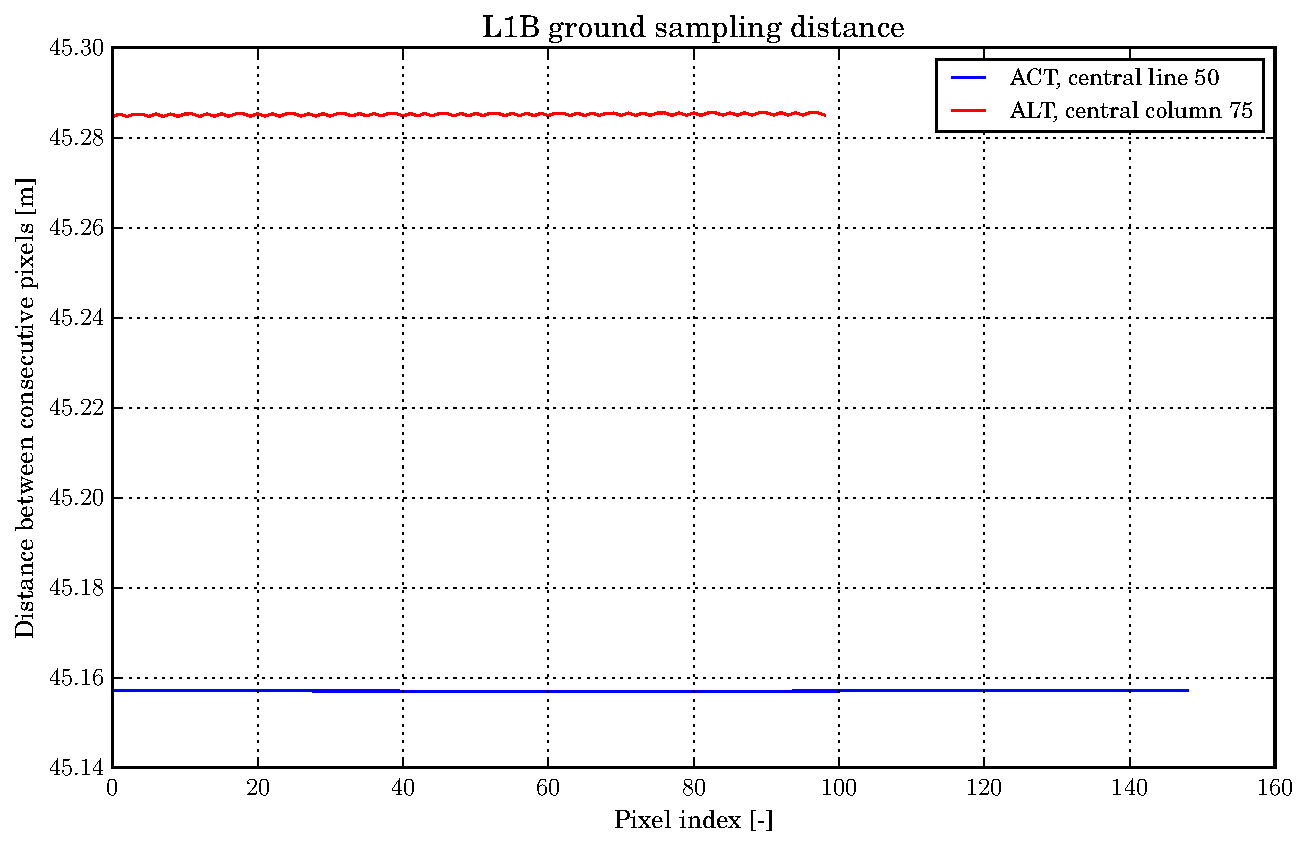
\includegraphics[width=0.75\textwidth]{l1c_gsd}
\caption{L1C. L1B ground sampling distance ACT and ALT.}
\label{fig:l1c_gsd}
\end{figure}

The GSD is about 45~m in both directions and it is almost constant over the scene.
Each L1B pixel covers about $45 \times 45 \approx 2045$~m$^2$. Each L1C tile covers $100 \times 100 = 10^4$~m$^2$.
The ratio is 4.9. Then $15000 / 4.9 \approx 3070$ tiles cover the scene. The rest of the 3129 tiles are on the borders, where tiles are only partly covered.

\subsubsection{L1C radiances}
Figures~\ref{fig:l1c_toa_0} to~\ref{fig:l1c_toa_3} compare the L1B and L1C radiances on the map.
The L1C keeps the gradient of the scene.
On the west border some L1C values differ from their neighbours. The south-west corner of these tiles is outside the L1B footprint, so the spline extrapolates. In VNIR-2 two points have a negative radiance for this reason.
A margin around the image or a check of the footprint would avoid it.

\begin{figure}[H]
\centering
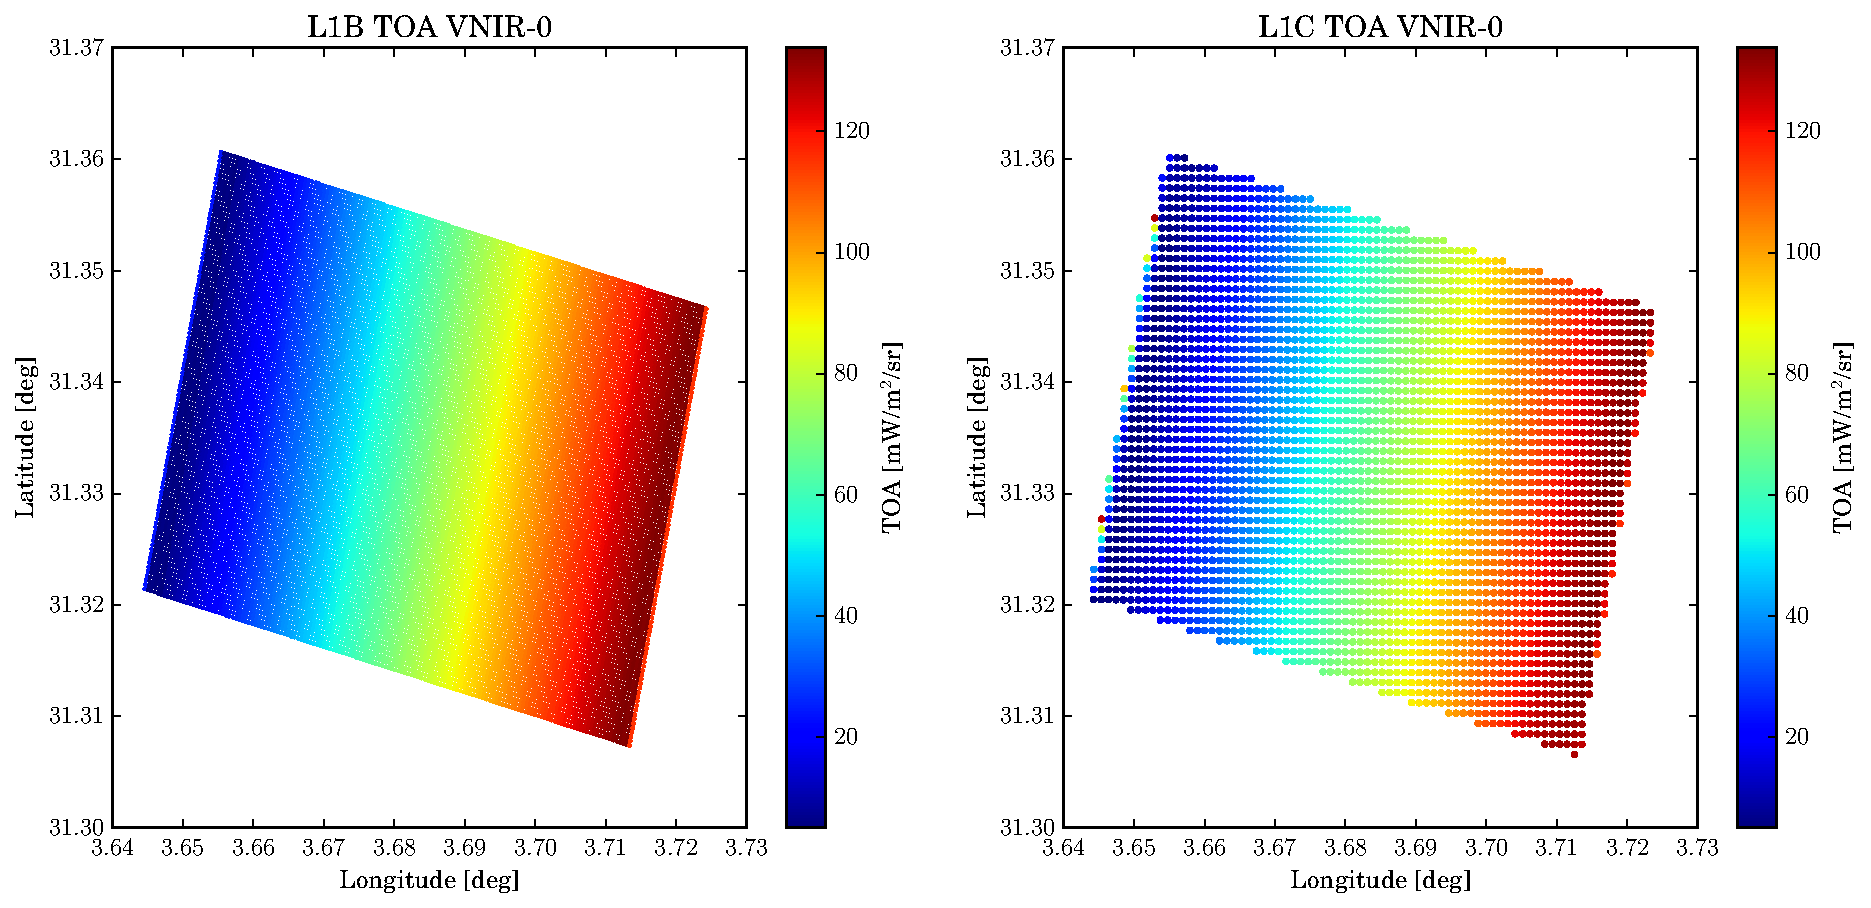
\includegraphics[width=\textwidth]{l1c_toa_map_VNIR-0}
\caption{L1C. L1B and L1C TOA, VNIR-0.}
\label{fig:l1c_toa_0}
\end{figure}

\begin{figure}[H]
\centering
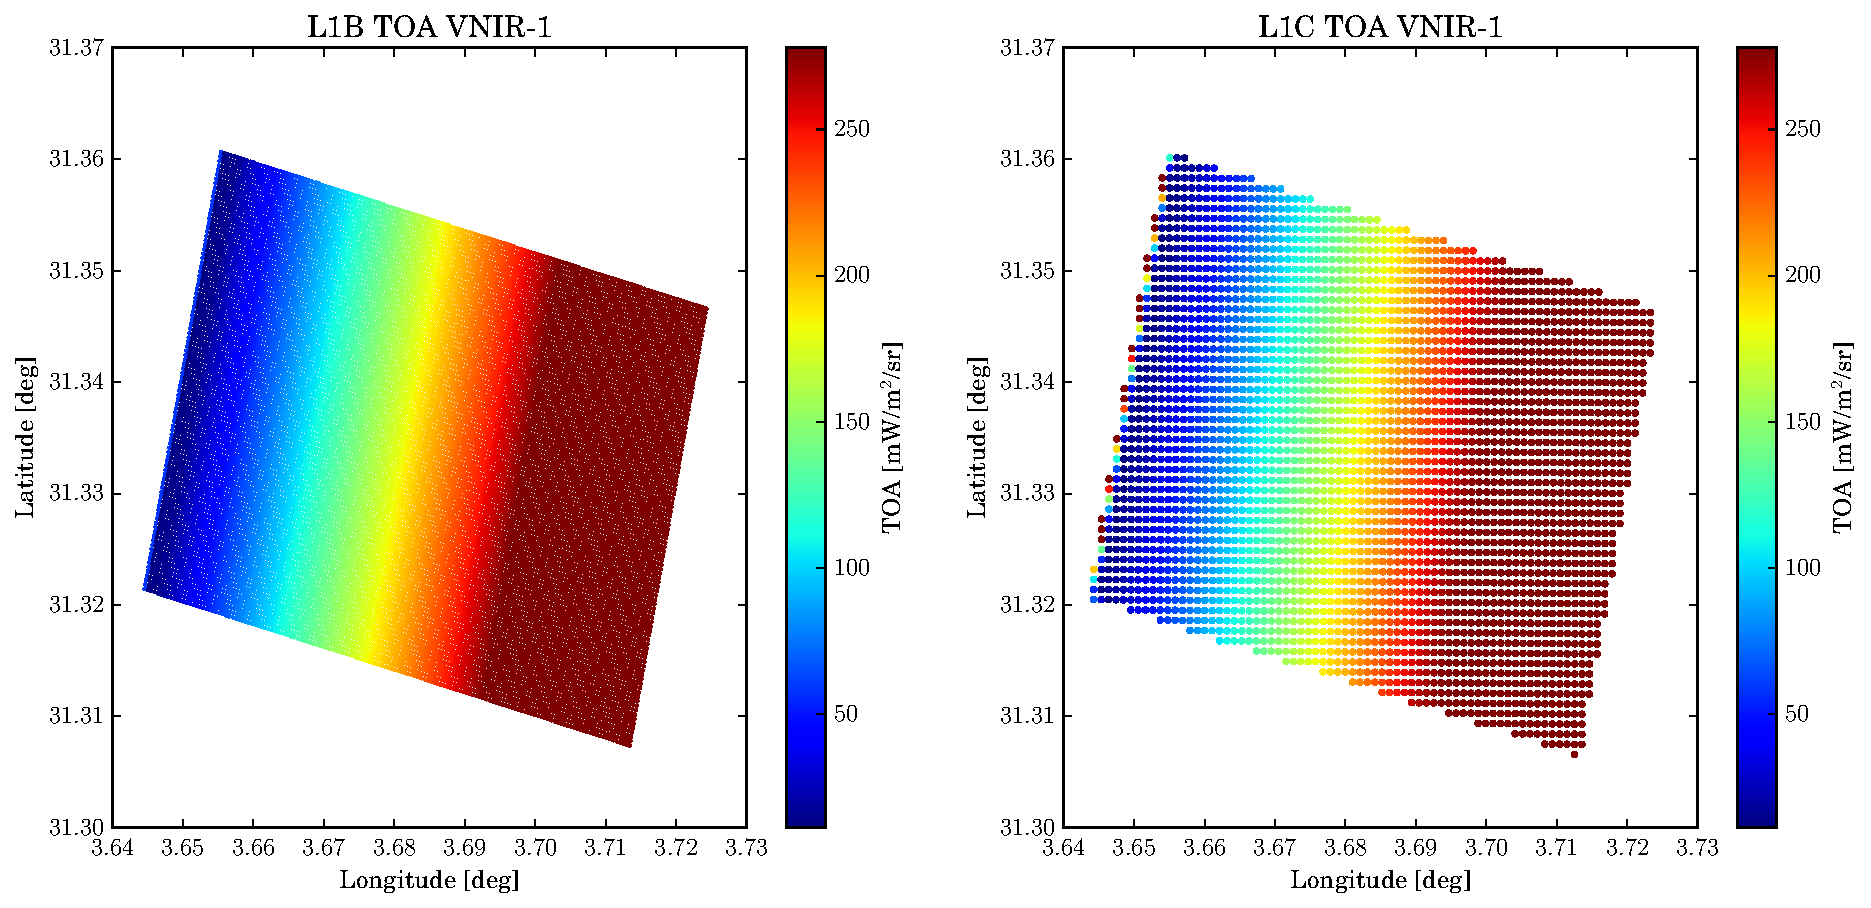
\includegraphics[width=\textwidth]{l1c_toa_map_VNIR-1}
\caption{L1C. L1B and L1C TOA, VNIR-1.}
\label{fig:l1c_toa_1}
\end{figure}

\begin{figure}[H]
\centering
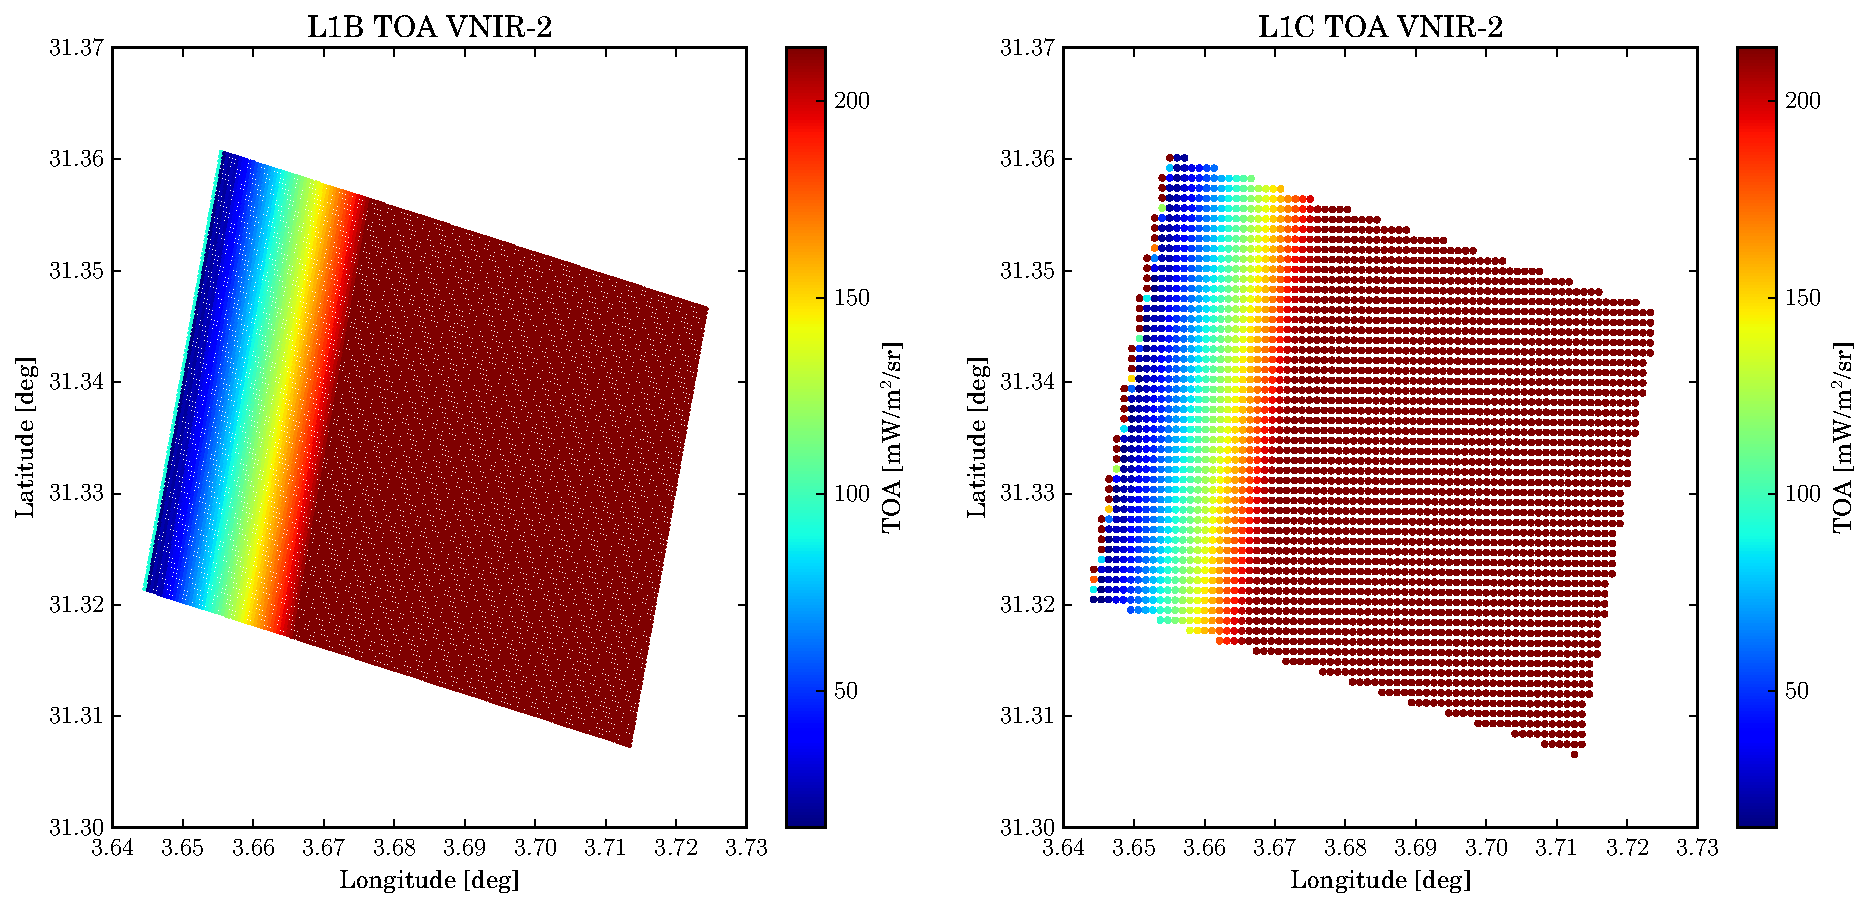
\includegraphics[width=\textwidth]{l1c_toa_map_VNIR-2}
\caption{L1C. L1B and L1C TOA, VNIR-2.}
\label{fig:l1c_toa_2}
\end{figure}

\begin{figure}[H]
\centering
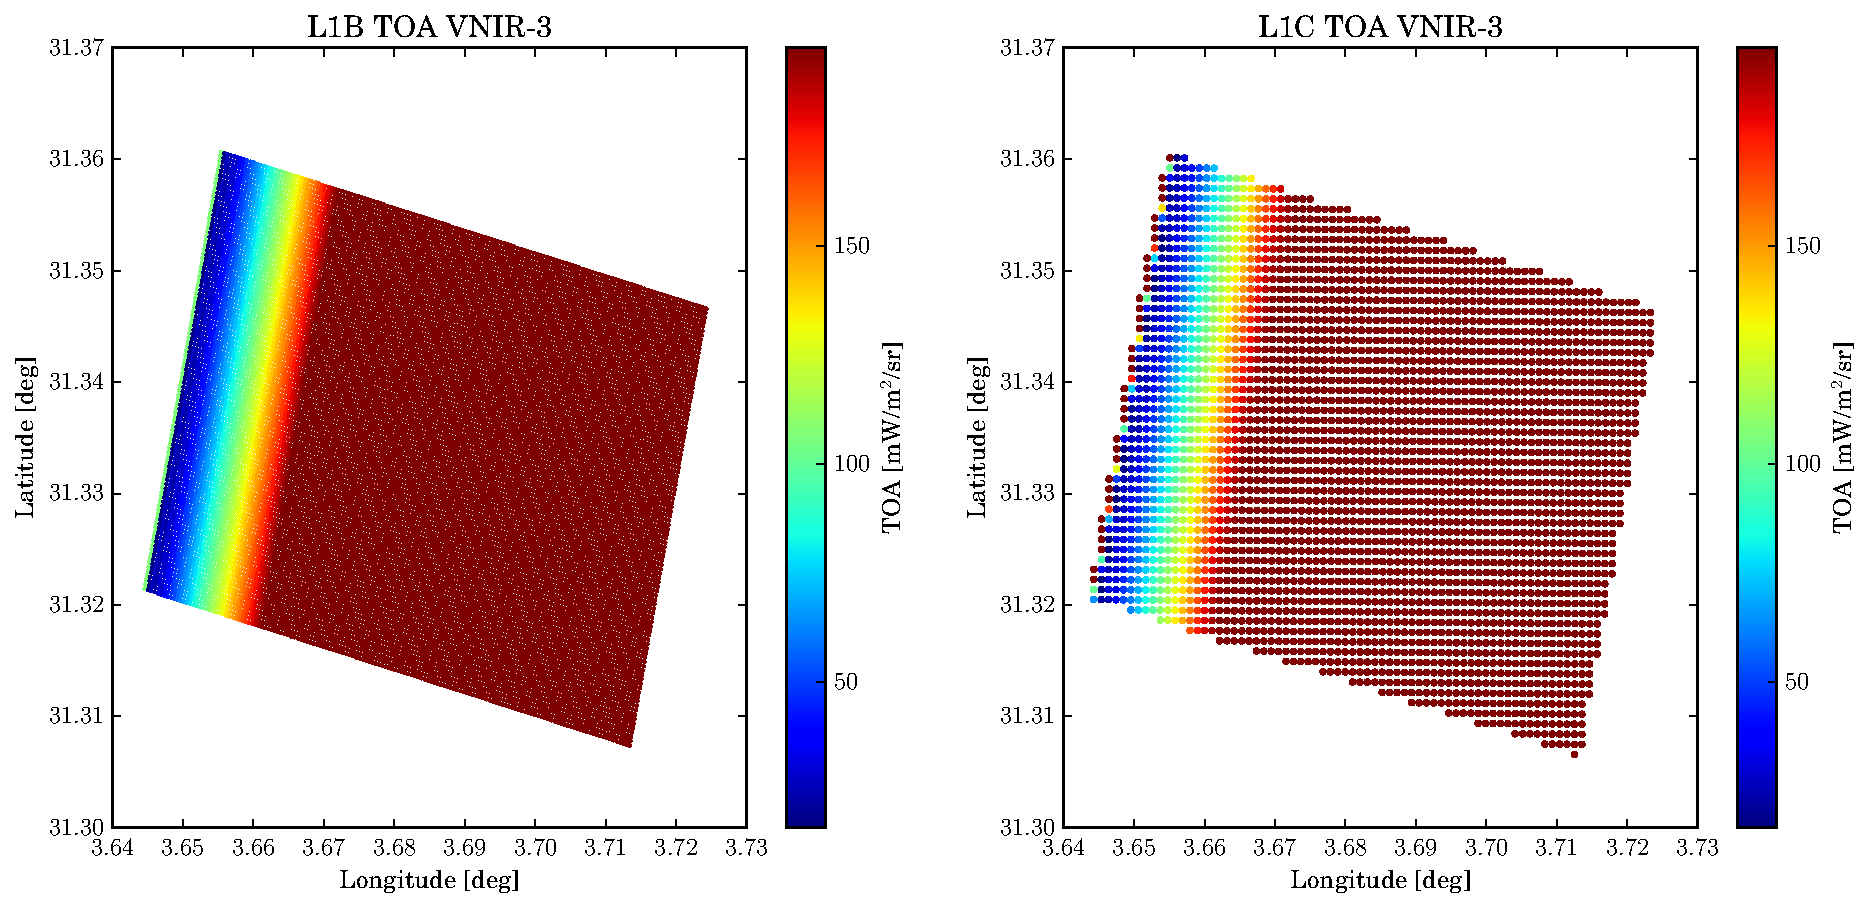
\includegraphics[width=\textwidth]{l1c_toa_map_VNIR-3}
\caption{L1C. L1B and L1C TOA, VNIR-3.}
\label{fig:l1c_toa_3}
\end{figure}

\subsection{Theoretical question. Processing levels and the need for the L1C}
The data of an EO mission are processed in levels.
\begin{itemize}
\item Level 0. Raw instrument packets in time order, as received on ground.
\item Level 1A. The packets are decoded into images in DN, with the time and the auxiliary data attached.
\item Level 1B. The DN are converted into radiances with the calibration. The image keeps the geometry of the sensor and each pixel has its geolocation.
\item Level 1C. The L1B radiances are resampled onto a fixed cartographic grid.
\item Level 2. Geophysical variables retrieved from the L1, such as reflectance, vegetation indices or fluorescence.
\end{itemize}

The L1B grid is different for each acquisition. It depends on the orbit, the attitude and the terrain.
Two L1B products of the same area cannot be compared pixel by pixel.
The L1C solves this. All the products are projected onto the same grid, so they can be stacked in time, combined with other sensors and used to build maps.
The L1B remains the most accurate radiance because it is not interpolated.

The grid used is the Military Grid Reference System (MGRS).
It is based on the UTM projection, which divides the Earth into 60 zones of $6^\circ$ in longitude. Each zone is a transverse Mercator projection with coordinates in metres.
MGRS divides each UTM zone into latitude bands of $8^\circ$ and squares of 100~km with two letters. Inside each square the easting and northing give the position. The number of digits fixes the precision.
In the code \texttt{31REQ660644} is zone 31, band R, square EQ, easting 660 and northing 644 in units of 100~m.

The L1C has fewer points than the L1B because the MGRS tile of 100~m is larger than the GSD of 45~m.
Several L1B pixels fall in the same tile and the tile is counted once.
The ideal grid size would be the SSD of the sensor. The configuration uses 100~m, as the ATBD recommends \cite{atbd}.

\subsection{Conclusion}
The L1C outputs match the reference after matching the points by coordinates.
The L1B GSD is 45.2~m ACT and 45.3~m ALT.
\textbf{EODP-TS-L1C: PASS.}
